\documentclass{article}
\usepackage{tikz, comment}
\usepackage{pifont}
\usepackage{fontspec, pgfplots}
\usetikzlibrary{arrows, decorations.markings, decorations.pathreplacing}
\begin{comment}
:Title: Not defined yet
:Tags: area using parametric equations,parametric integral formula;directrices of a hyperbola;moment;focus of a parabola;x-y plane
:Prob: 0.5722;0.5715;0.5538;0.5381;0.5368
:Author: Prof.Hu Ji-shan, HKUST
:Slug: No name yet

Description Here.........
\end{comment}
\begin{document}\centering 

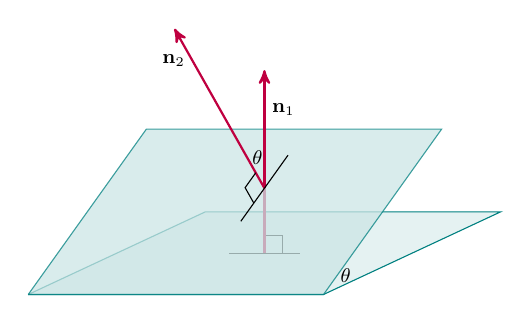
\begin{tikzpicture}[>=latex,xscale=.5*1.5, yscale=.5*1.5][font=\sf\small] 

\draw[teal, fill=teal!10] (0, 0)--++(5, 0)--++(3, 1.4)--++(-5, 0)--++(-3,-1.4);

\node[xshift=8, yshift=7, scale=0.8] at (5, 0) {$\theta$};

\draw ({4-0.6}, 0.7)--++(1.2, 0);

\draw ({4+0.3}, 0.7)--++(0, 0.3)--++(-0.3, 0);

\draw[purple, thick] ({4}, 0.7)--++(0, 2.7) node[black, right, pos=0.9, scale=0.8] {${\bf n}_1$};

\draw[teal, fill=teal!20, opacity=0.75] (0, 0)--++(5, 0)--++(2, 2.8)--++(-5, 0)--++(-2,-2.8);

\draw[purple, thick, ->, >=stealth'] (4, 1.8)--++(0, 2.0);

\draw[purple, thick, ->, >=stealth'] (4, 1.8)--++({-(2.0+1.1)*sin(0.51392 r)}, {(2.0+1.1)*cos(0.51392 r)}) node[black, left, pos=0.8, scale=0.8] {${\bf n}_2$};

\node[xshift=-2.5, yshift=11, scale=0.8] at (4, 1.8) {$\theta$};

\draw[samples=100, smooth, domain=4-0.4:4+0.4, variable=\x] 
		plot ({\x}, {1.8+2.8/2*(\x-4)}); 

\draw ({4-0.18}, {1.8+2.8/2*(4-0.18-4)})--++({-0.3*sin(0.51392 r)}, {0.3*cos(0.51392 r)})--({4-0.3*sin(0.51392 r)}, {1.8+0.3*cos(0.51392 r)});
		
\end{tikzpicture}
\end{document}